\chapter{Stand der Forschung und Stand der Technik}

Das Projekt ist eine pädagogische Umsetzung für Pflege Studenten im Bereich E-Learning mit aktuelle Web Technologie. Das Konzept des Projektes basiert auf den Theorien über E-Learning und VR-Training. Und die Implementierung des Projektes profitiert von der Entwicklung der Technik Virtuelle Realität (VR), beziehungsweise im Fachbereich WebVR.

\section{Stand der Forschung}

Als die theoretische Unterstützung dieses Projektes wird der Stand der Forschung von E-Learning und VR-Training erzählt.

 \subsection{E-Learning}
 E-Learning ist kein neuer Begriff, jedoch ist es nicht einfach, eine allumfassende Definition zu finden, weil E-Learning mit vielfältigen Fächern verbindet. Je nach Schwerpunkt fallen die jeweiligen Definitionen unterschiedlich aus.

E-Learning umfasst laut Kerres \citep{1} \glqq bei denen elektronische oder digitale Medien für die Präsentation und Distribution von Lernmaterialien und/oder Unterstützung zwischenmenschlicher Kommunikation zum Einsatz kommen.\grqq

Die Entwicklung der Web Technologie von \glqq Web 1.0\grqq\ zu \glqq Web 2.0\grqq\  \citep{3}, nämlich von \glqq the Read Web \grqq\ zu \glqq the Read-Write Web\grqq\ \citep{4} bietet mehr technische Möglichkeiten für E-Learning. Stephen Downes \citep{2} bezeichnet E-Learning ab 2005 als E-Learning 2.0. Da \glqq entwickelt sich E-Learning mit dem World Wide Web als Ganzes weiter und ändert sich so stark, dass ein neuer Name entsteht.\grqq\

In dieser Arbeit wird der Begriff E-Learning als Synonym des E-Learnings 2.0, erfahrungsgemäß Online Learning benutzt.
 
Zurzeit bezieht Internet sich auf notwendige Infrastruktur, deren Geschwindigkeit, Stabilität und Mobilität immer verbessert werden. Die Form des Rechners ist auch unterschiedlich, Desktop, Laptop, Tablet, Smartphone und VR Geräte. Die entwickelte Technik garantiert die stabile und vielfältige Nutzung von E-Learning. Im Jahr 2013 haben 35\% der Deutschen E-Learning-Erfahrung. (Abbildung ~\ref{fig:eLearningErfahrung})

\begin{figure}[ht]
\vspace*{1em}
\centering
\caption[E-Learning-Erfahrung]{E-Learning-Erfahrung}
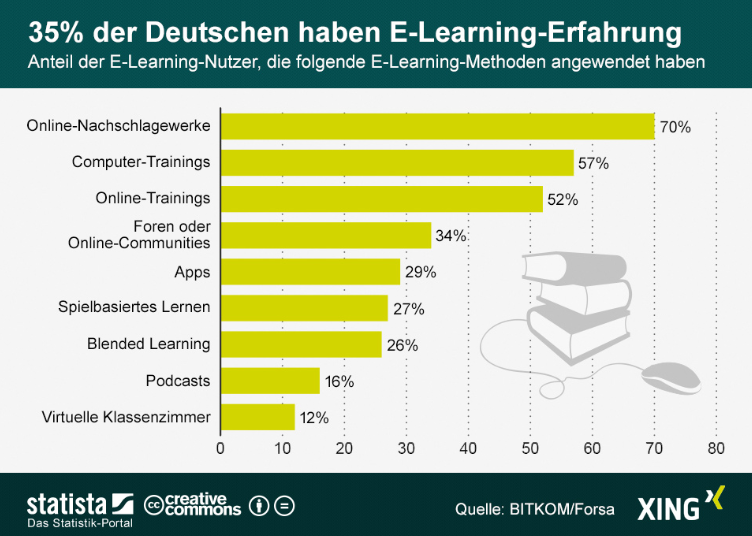
\includegraphics[width=\textwidth]{images/eLearningErfahrung.png}
\label{fig:eLearningErfahrung} 
\end{figure}

Laut der Statistik ist die prognostische Umsätze durch E-Learning weltweit von 2016 bis 2021 mehr als 30.000 Millionen US-Dollar jedes Jahr. (Abbildung ~\ref{fig:umsatzDiagnose})

\begin{figure}[ht]
\vspace*{1em}
\centering
\caption[E-Learning Umsatz Diagnose]{E-Learning Umsatz Diagnose}
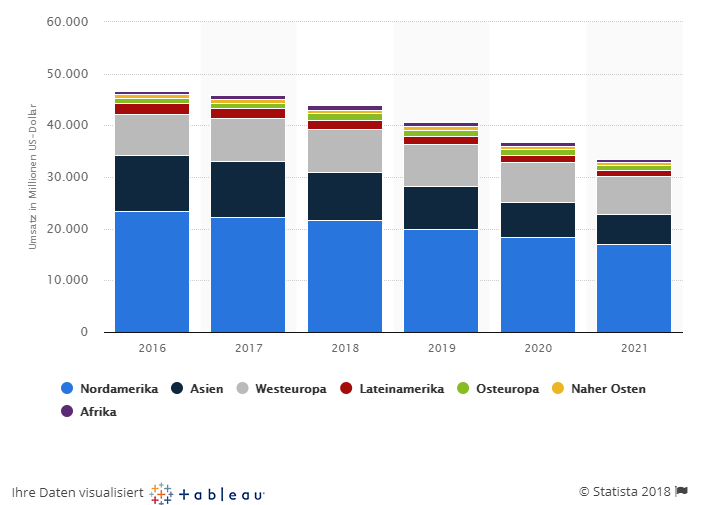
\includegraphics[width=\textwidth]{images/umsatzDiagnose.png}
\label{fig:umsatzDiagnose} 
\end{figure}

E-Learning ist schon ein unverzichtbares pädagogisches Mittel mit hochwertiger wirtschaftlicher Markt. Und auf dem E-Learning Markt spielt die Hochschulen eine entscheidende Rolle. (Abbildung ~\ref{fig:zielgruppe})

\begin{figure}[ht]
\vspace*{1em}
\centering
\caption[E-Learning Verbrauchergruppe]{E-Learning Verbrauchergruppe}
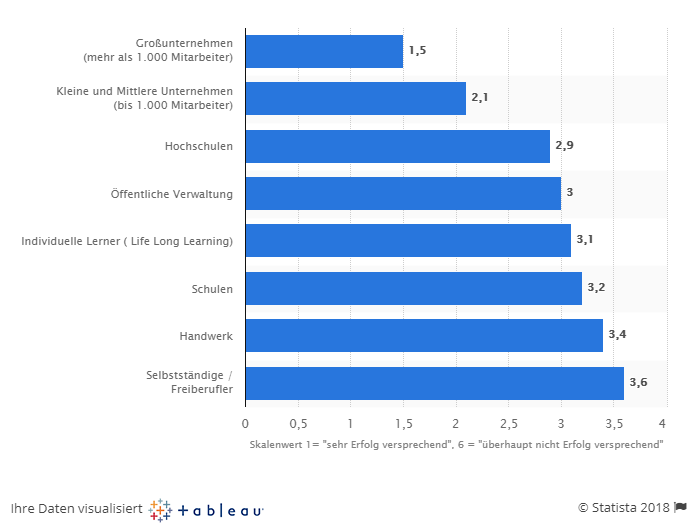
\includegraphics[width=\textwidth]{images/zielgruppe.png}
\label{fig:zielgruppe} 
\end{figure}

Als ein wichtiges Werkzeug im Bereich Ausbildung sind sieben Merkmale des E-Learnings laut Justin Ferriman \citep{6} eindeutig:

\begin{enumerate}
\item Skalierbarkeit: Inhaltliche Änderung gehen schnell. 
\item Kapazität und Konsistenz: Pädagogen können eine große Reichweite für ihre Zielgruppe erreichen und die Botschaft wird auf konsistente Weise kommuniziert.
\item Hohe Aufbewahrung: Vielfältige Learning-Ansätze führen dazu, dass Inhalte besser gemerkt werden können.
\item Zeitliche und finanzielle Ersparnisse: E-Learning entfernt die Bedürfnisse der Reise und Stelle.
\item Aktivitäts- und ROI (Return On Investment)-Messungen: Das Erfassen des Lernfortschritts und die Berichterstellung der Lernaktivitäten sind mühelos und anschaulich.
\item Reduzierung von CO2-Fußabdruck: Wenige Reisen und weniger Bedarf an papierlichen Ausdrücken reduziert der Kohlendioxid-Ausstoß.
\item Flexibilität: Es gibt keine zeitliche oder geografische Begrenzung für die Studenten.
\end{enumerate}\

Um bessere E-Learning Projekt zu entwickeln, müssen die Nachteile des E-Llearnings identifiziert werden. Im Jahr 2011 haben Mair Angelika und Butzerin Janine \citep{7} elf Nachteile von E-Learning aufgelistet. Obwohl nach sieben Jahren im Jahr 2018 einige Mängel z.B. \glqq Das Angebot an Qualitätsprodukten am Markt ist Überschaubar \grqq\ nicht sehr angepasst sind, sind viele Auffassungen nach wie vor sinnvoll.

\begin{enumerate}
\item Technische Abhängigkeit: Rechner und Internet sind die Grundlage des E-Learnings, und mehr neue Technik wird zu Verfügung stehen, z.B. VR und AR (augmented reality).
\item Kein sozialer Kontakt: Obwohl Chat-Rooms, video conferencing sogar VR meeting werden in E-Learning eingesetzt, ist der direkte menschliche Kontakt nicht ersetzbar.
\item Mangelnde praktische Teile: Die praktischen Übungen im Labor sind besonders schwierig mit E-Learning durchzuführen.
\item Disziplin und Selbstlernkompetenz: Die Motivation und die Kontinuität können nicht garantiert werden.
\end{enumerate}\

Noch ein nachteiliger Punkt, den von Richard Nolan \citep{5} nennt, kann als eine Ergänzung gelten. Das Feedback kommt nicht ausführlich genug bzw rechtzeitig. Aufgrund der zeitlichen Freiheit des E-Learnings können die Studenten jederzeit lernen, außerdem kann die Zahl der Lernenden sehr umfangreich sein, deswegen wird das rechtzeitige Feebacks, besonders die Antwort der individuellen Fragen nicht sichergestellt.

Das E-Learning wird schon häufig verwendet, aber ist es wirklich effektiver und effizienter als traditionelle pädagogische Mittel, die im Klassenzimmer genutzt werden? Um die Frage zu beantworten, hat Will Thalheimer \citep{8} eine Metaanalyse durchgeführt. Die Lernmethoden, beispielsweise Karteikarten, Brainstorming und Tests, gelten als Einflussfaktoren im Vergleich zwischen den Modalitäten des Lernens, nämlich E-Learning und der Unterricht im Klassenzimmer. Aus der Untersuchung mit 28 Arbeiten ergibt sich die Folgerung:

\begin{enumerate}
\item Wenn die Lernmethoden gleichbleibend sind, produzieren beide das gleiche Ergebnis.
\item Wenn die Lernmethoden nicht gleich sind, dann übertrifft E-Learning den Unterricht im Klassenzimmer.
\item Der Effekt von E-Learning kann besser, schlechter, manchmal auch gleich wie der Effekt des Unterrichts im Klassenzimmer sein.
\item Die Modalitäten des Lernens spielen keine wichtige Rolle für den Lerneffekt, sondern die Lernmethoden wie realistische Praxis, Wiederholung in zeitlichen Abständen, realer Kontext und Feedback.
\item Die Mischung mit E-Learning und dem Unterricht im Klassenzimmer erzielt die beste Wirkung. Wahrscheinlich ist der Grund, dass mehr effektive Lernmethoden eingesetzt werden können. 
\end{enumerate}\

Zusammenfassung der Forschung kann sein, dass der größte Vorteil des E-Learnings ist, mehr effektive Lernmethoden anzubieten.

Dank der schnell entwickelnden Web Technik werden mehr Lernmethoden ermöglicht. In dem Bericht \glqq Elearning market trends and forecast 2017 -2021\grqq\ von Docebo werden die fünf wichtigsten Technologien aufgelistet, die mit E-Learning integriert werden. Die Anwendung dieser Technologien wird die Effektivität und die Effizienz des E-Learnings verbessern. (Abbildung ~\ref{fig:elearningtop5technology})

\begin{figure}[ht]
\vspace*{1em}
\centering
\caption{Top 5 Prioritäten für Lerntechnologien}
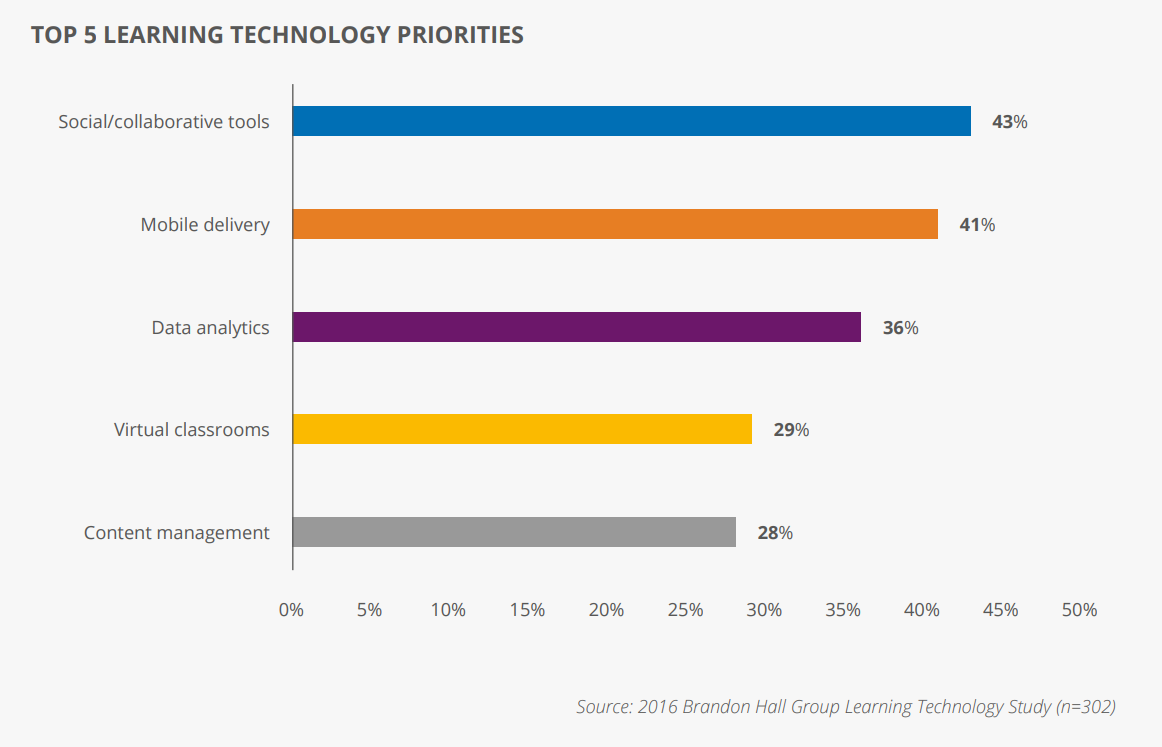
\includegraphics[width=\textwidth]{elearningtop5technology}
\label{fig:elearningtop5technology} 
\end{figure}

Fast ein Drittel der gefragten Unternehmen finden, dass der virtuelle Klassenraum ein hilfreiches Werkzeug für die Schulung sein wird.

 \subsection{VR-Training}
 
Virtuelle Realität (VR) ist die Technik, die die Situation \glqq Interaktiv erzeugte multimodale Sinneseindrücke 2. Ordnung, die von Menschen als solche 1. Ordnung wahrgenommen werden.\grqq\ \citep{9} realisiert. Kurz gefasst: mit VR Technik wird der Nutzer in einer virtuellen Umgebung eingebracht. (Abbildung ~\ref{fig:vrhtcvive})


\begin{figure}[ht]
\vspace*{1em}
\centering
\caption{Virtuelle Realität}
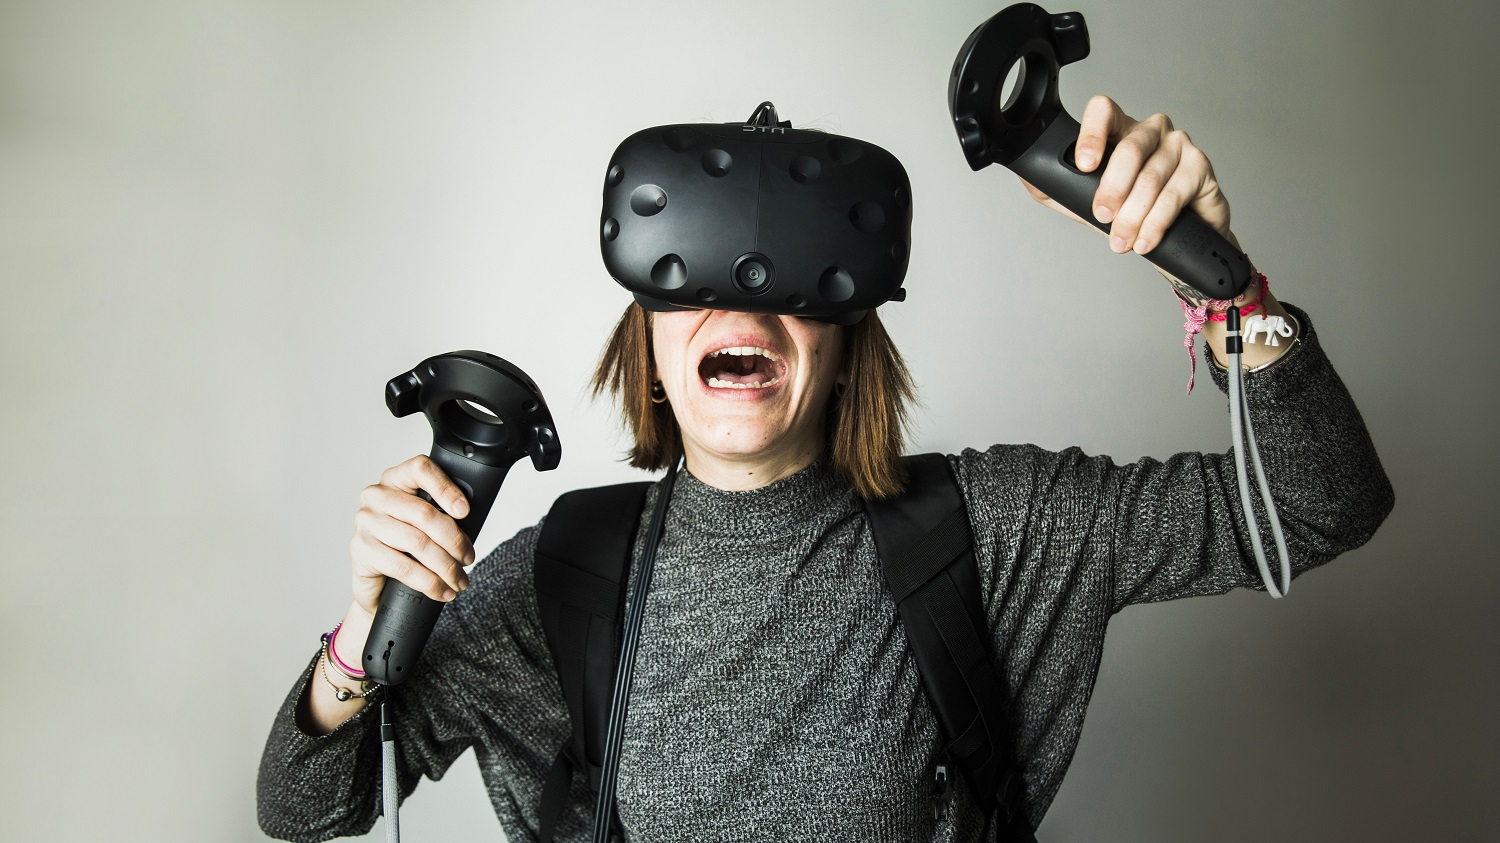
\includegraphics[width=\textwidth]{images/vrhtcvive.jpg}
\label{fig:vrhtcvive} 
\end{figure}

VR-Training ist ein Synonym des virtual reality-based training (VRBT). \glqq VRBT ist eine interaktive und umfassende Unterrichtsmethode, bei der mithilfe von Technologien virtuelle Szenarien bereitgestellt werden, um Situationen zu simulieren, die in tatsächlichen Umgebungen auftreten können. \grqq\ \citep{14} 
Das immersive Erleben zeugt davon, dass die VR Technik gut geeignet für Training ist.

Laut der Forschung von James Clark und Allan Paivio \citep{10} wird die Gedächtnisleistung verstärkt, wenn multisensorische und emotionale Wahrnehmungen mit eingebracht werden. Die Forschung von S.A. Christianson \citep{11} stimmt überein, dass je stärker eine emotionale Reaktion auf einen Reiz ist, desto stärker das Gedächtnis darauf reagiert. 

\glqq VR ist ein wirksames Medium zur Stimmungsinduktion, das seinen Einsatz in verschiedenen Anwendungsbereichen eröffnet, die von der Wohlbefinden-Branche bis zur klinischen Psychologie reichen. \grqq\ \citep{29} Was noch wichtig ist, ist, dass das simulierte Szenario wiederholbar und die dargestellte emotionale und stressige Situation kontrollierbar ist, deswegen wird VR eine wichtige Rolle im Bereich der neurowissenschaftlichen Forschung und Therapie spielen \citep{13}. Laut der Forschung von Albert A. Rizzo kann die VR Technik zudem als Hilfsmittel bei der Behandlung von Phobien benutzt werden \citep{12}. 

Eine Studie \citep{30} beweist, dass VR die Gedächtnisleistung fördert. Die Probanden werden in zwei Gruppen aufgeteilt. Eine Gruppe schaut sich ein Video in 2D an. Die andere Gruppe schaut ein 360\degree\ Video, deren Inhalt identisch zu dem 2D Video ist. Der einzige Unterschied sind die 360\degree\ und die damit verbundene Notwendigkeit des Tragens einer VR Brille. Nach 48 Stunden kann sich die VR Gruppe besser an der Inhalte des Videos erinnern, als die 2D Gruppe.

Im Buch \glqq The VR Book: Human-Centered Design for Virtual Reality \grqq\ \citep{28} wird die Immersion in sechs Kategorien eingeteilt: 

\begin{enumerate}
\item \textbf{Extensiveness} beschreibt die Stärke und Menge der angesprochenen Sinne (z.B Optik, Akustik).
\item \textbf{Matching} erfasst die Anpassung des Feedbacks in einer virtuellen Umgebung für die Interaktion (z.B Übertragung der Kopfbewegungen).
\item \textbf{Surroundness} ist die räumliche Repräsentation (z.B Blickfeld, räumlicher Sound).
\item \textbf{Vividness} erfasst die technische Implementierung einer Simulation (z.B bildliche Auflösung, Materialienauswahl, Texturen)
\item \textbf{Interactability} beschreibt die Möglichkeiten der Interaktion, um die Objekten in einer virtuellen Umgebung zu beeinflussen (z.B klicken, drücken)
\item \textbf{Plot} beschreibt das Verhalten, das nach den physikalischen Gesetzen in der realen Welt in virtuelle Umgebung nachgeahmt wird.
\end{enumerate}\

Durch die Studie von Doug A. Bowman \citep{27} konnte herausgefunden werden, dass eine bessere Immersion zu einem besseren räumlichen Verständnis beiträgt und zu höherer Leitung bei interaktiven Aufgaben führen kann.

Als neue technische Anwendung im Bereich Schulung hat VR-Training viele herausragende Vorteile \citep{15}:

\begin{enumerate}
\item VR macht Schulung visueller: die immersive Darstellung eines 3D Szenarios in VR ist visueller und attraktiver als 2D Darstellungen, wie Videos, Bilder und Texte.
\item VR macht Schulung sicherer: in vielen Arbeitsbereichen wie Fertigung, Energie und Verteidigung sind Unfälle während der Schulung nur schwer zu vermeiden. Mithilfe der VR Technik können die Praxisphasen in einer virtuellen Umgebung simuliert und durchgeführt werden, was das Risiko der Unfälle minimiert.
\item VR macht Schulung erschwinglicher: die Kosten für Schulungen können sehr teuer sein, besonders wenn die Materialien nicht wiederverwendbar sind und es somit zu einem hohen Verbrauch und hohen Materialienkosten führt. Abgesehen von den Ausgaben für VR Geräte und die Entwicklung kostet VR-Training im Vergleich nur wenig Geld.
\item VR macht mehr Fernschulung möglich: durch die VR Technik können vielen Praxisphasen auch zuhause durchgeführt werden, ohne dass die Anwesenheit in speziellen Vorrichtungen und die Aufsicht einer Lehrperson von Nöten ist.
\item VR macht Aufbewahrung und Rückruf der Schulung möglich: durch VR Technik kann der Trainingsverlauf gespeichert werden, und es können bestimmte Aufgaben separat angesteuert und gezielt trainiert werden.
\end{enumerate}\

Die Auffassung von SIMBLOG \citep{16} beinhaltet weitere Vorteile, die hier ergänzt werden können:

\begin{enumerate}
\item Komplexe Probleme und Situationen vereinfachen: mithilfe der VR Technik können komplexe Situation und Abläufe in kleinere Abschnitte gegliedert werden, sodass diese im einzelnen angesteuert werden können.
\item Mehr Spaß: durch sogenannte \glqq Gamification\grqq\ können nachgebaute Szenarien aus der echten Welt einen spielerischen Charakter erhalten, was die Attraktivität der Übungen steigern und zu vermehrterem motivierterem Training führen kann.
\end{enumerate}\

Ein weiterer bedeutsamer Vorteil ist, dass bei jedem Trainingsdurchlauf in VR gewisse Daten gespeichert werden können, die eine Dokumentation des Trainingsverlaufs ermöglichen (Abbildung ~\ref{fig:intentionanalys1} \& Abbildung ~\ref{fig:intentionanalys2}). So können gewisse Schwierigkeiten im Training ermittelt und gezielt wiederholt werden, was zu einer verbesserung des Trainingsverlaufs und Lerneffekts führt. \glqq Oft ist es schwierig oder unmöglich, die Leistung zu verbessern, ohne die zugrunde liegenden kognitiven Faktoren zu kennen, die die Leistung beeinflussen. Die einzigartige, von STRIVR entwickelte VR-Aufmerksamkeitsanalyse ermöglicht diesen Einblick.\grqq\ \citep{18}

\begin{figure}[ht]
\vspace*{1em}
\centering
\caption{Aufmerksamkeit Analyse}
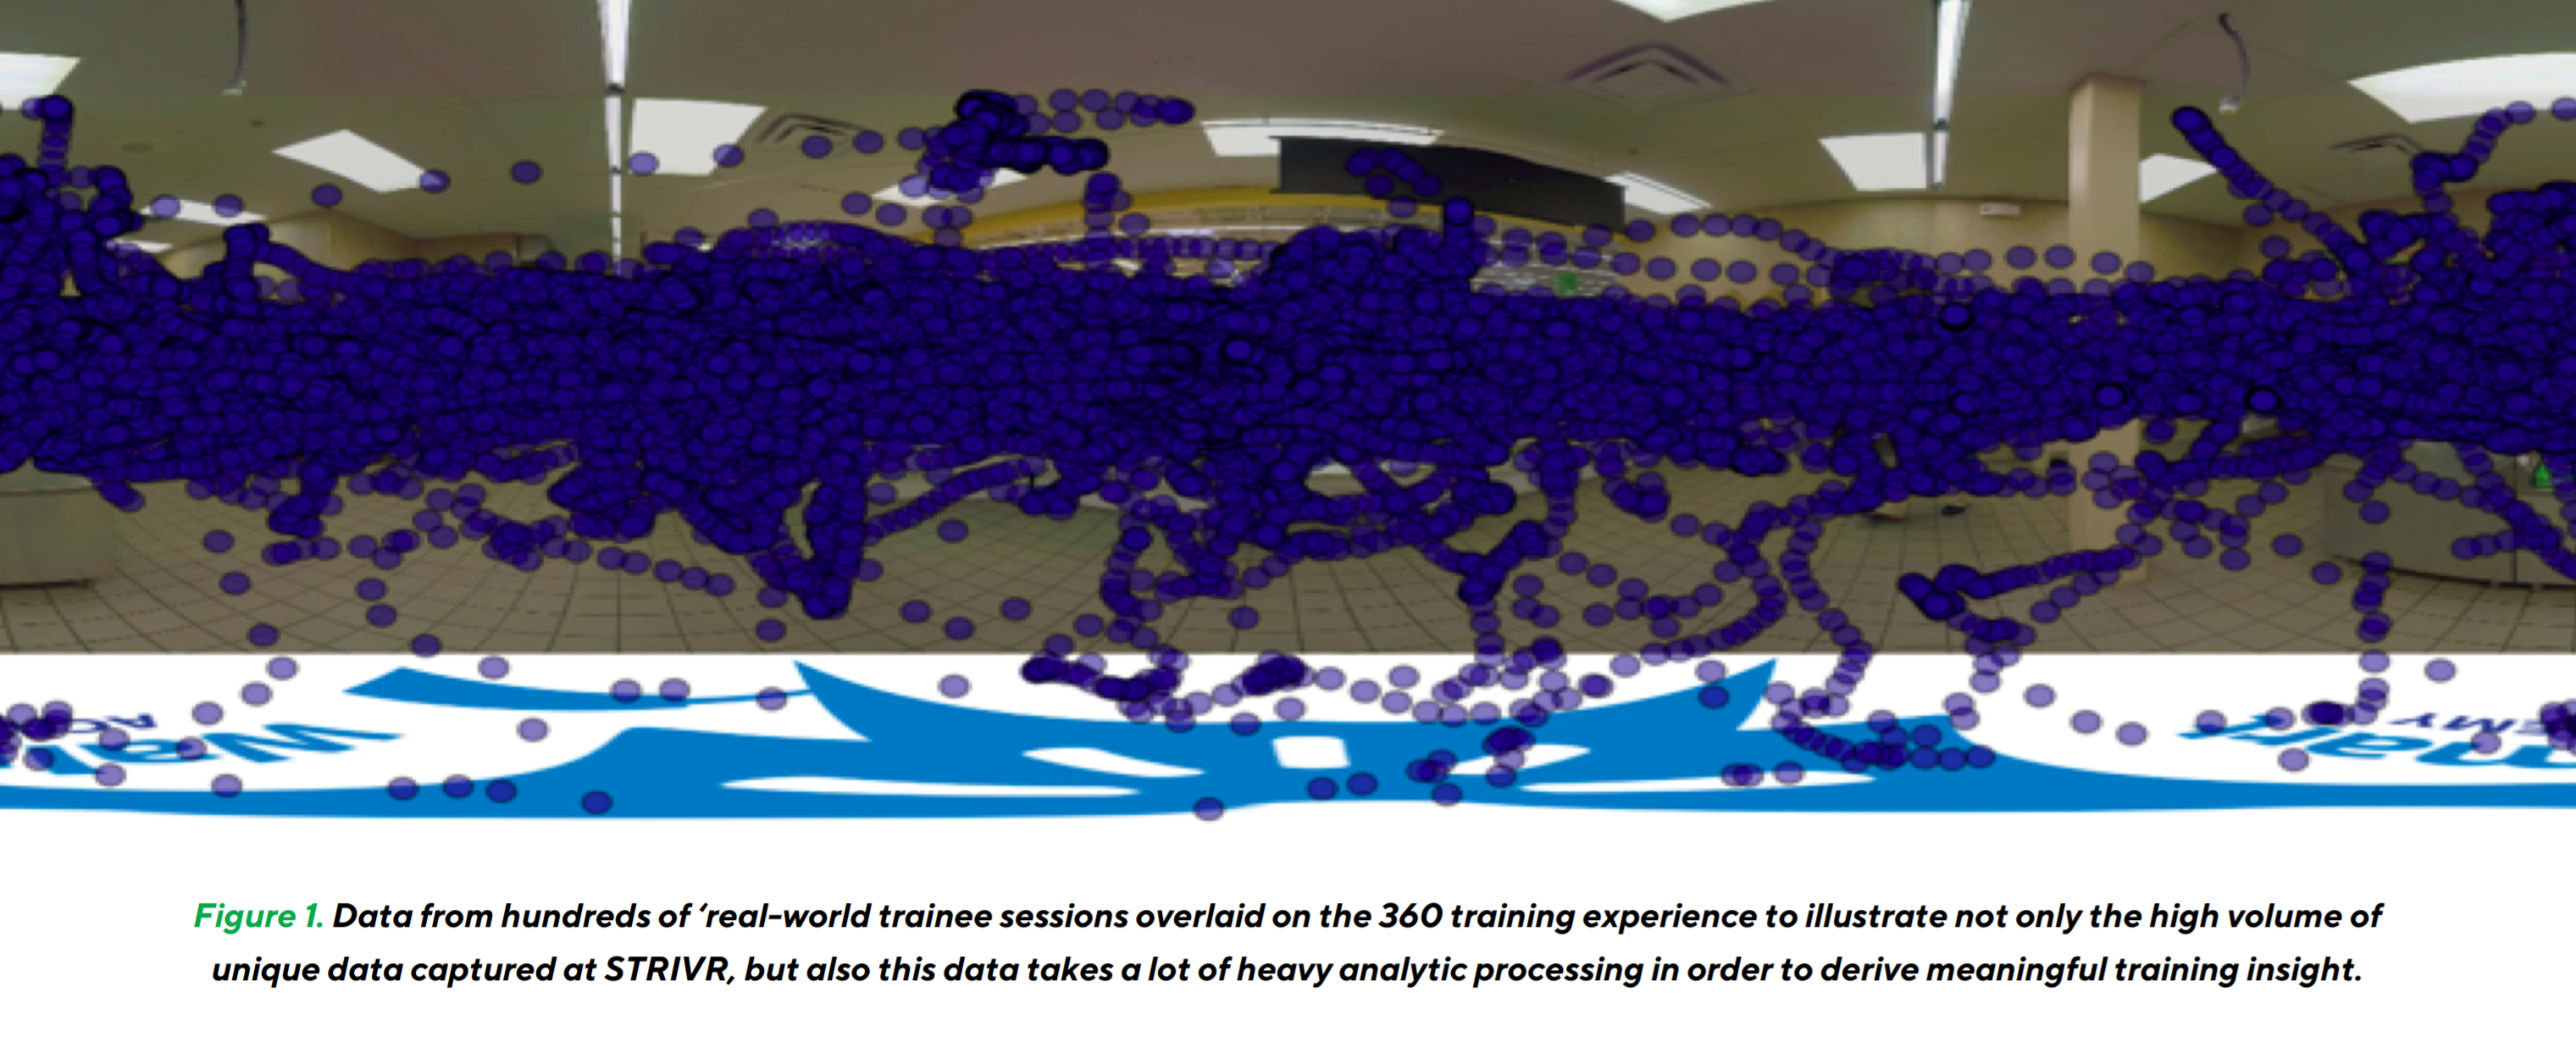
\includegraphics[width=\textwidth]{images/intentionanalys1.png}
\label{fig:intentionanalys1}
\end{figure}

\begin{figure}[ht]
\vspace*{1em}
\centering
\caption{Aufmerksamkeit Analyse}
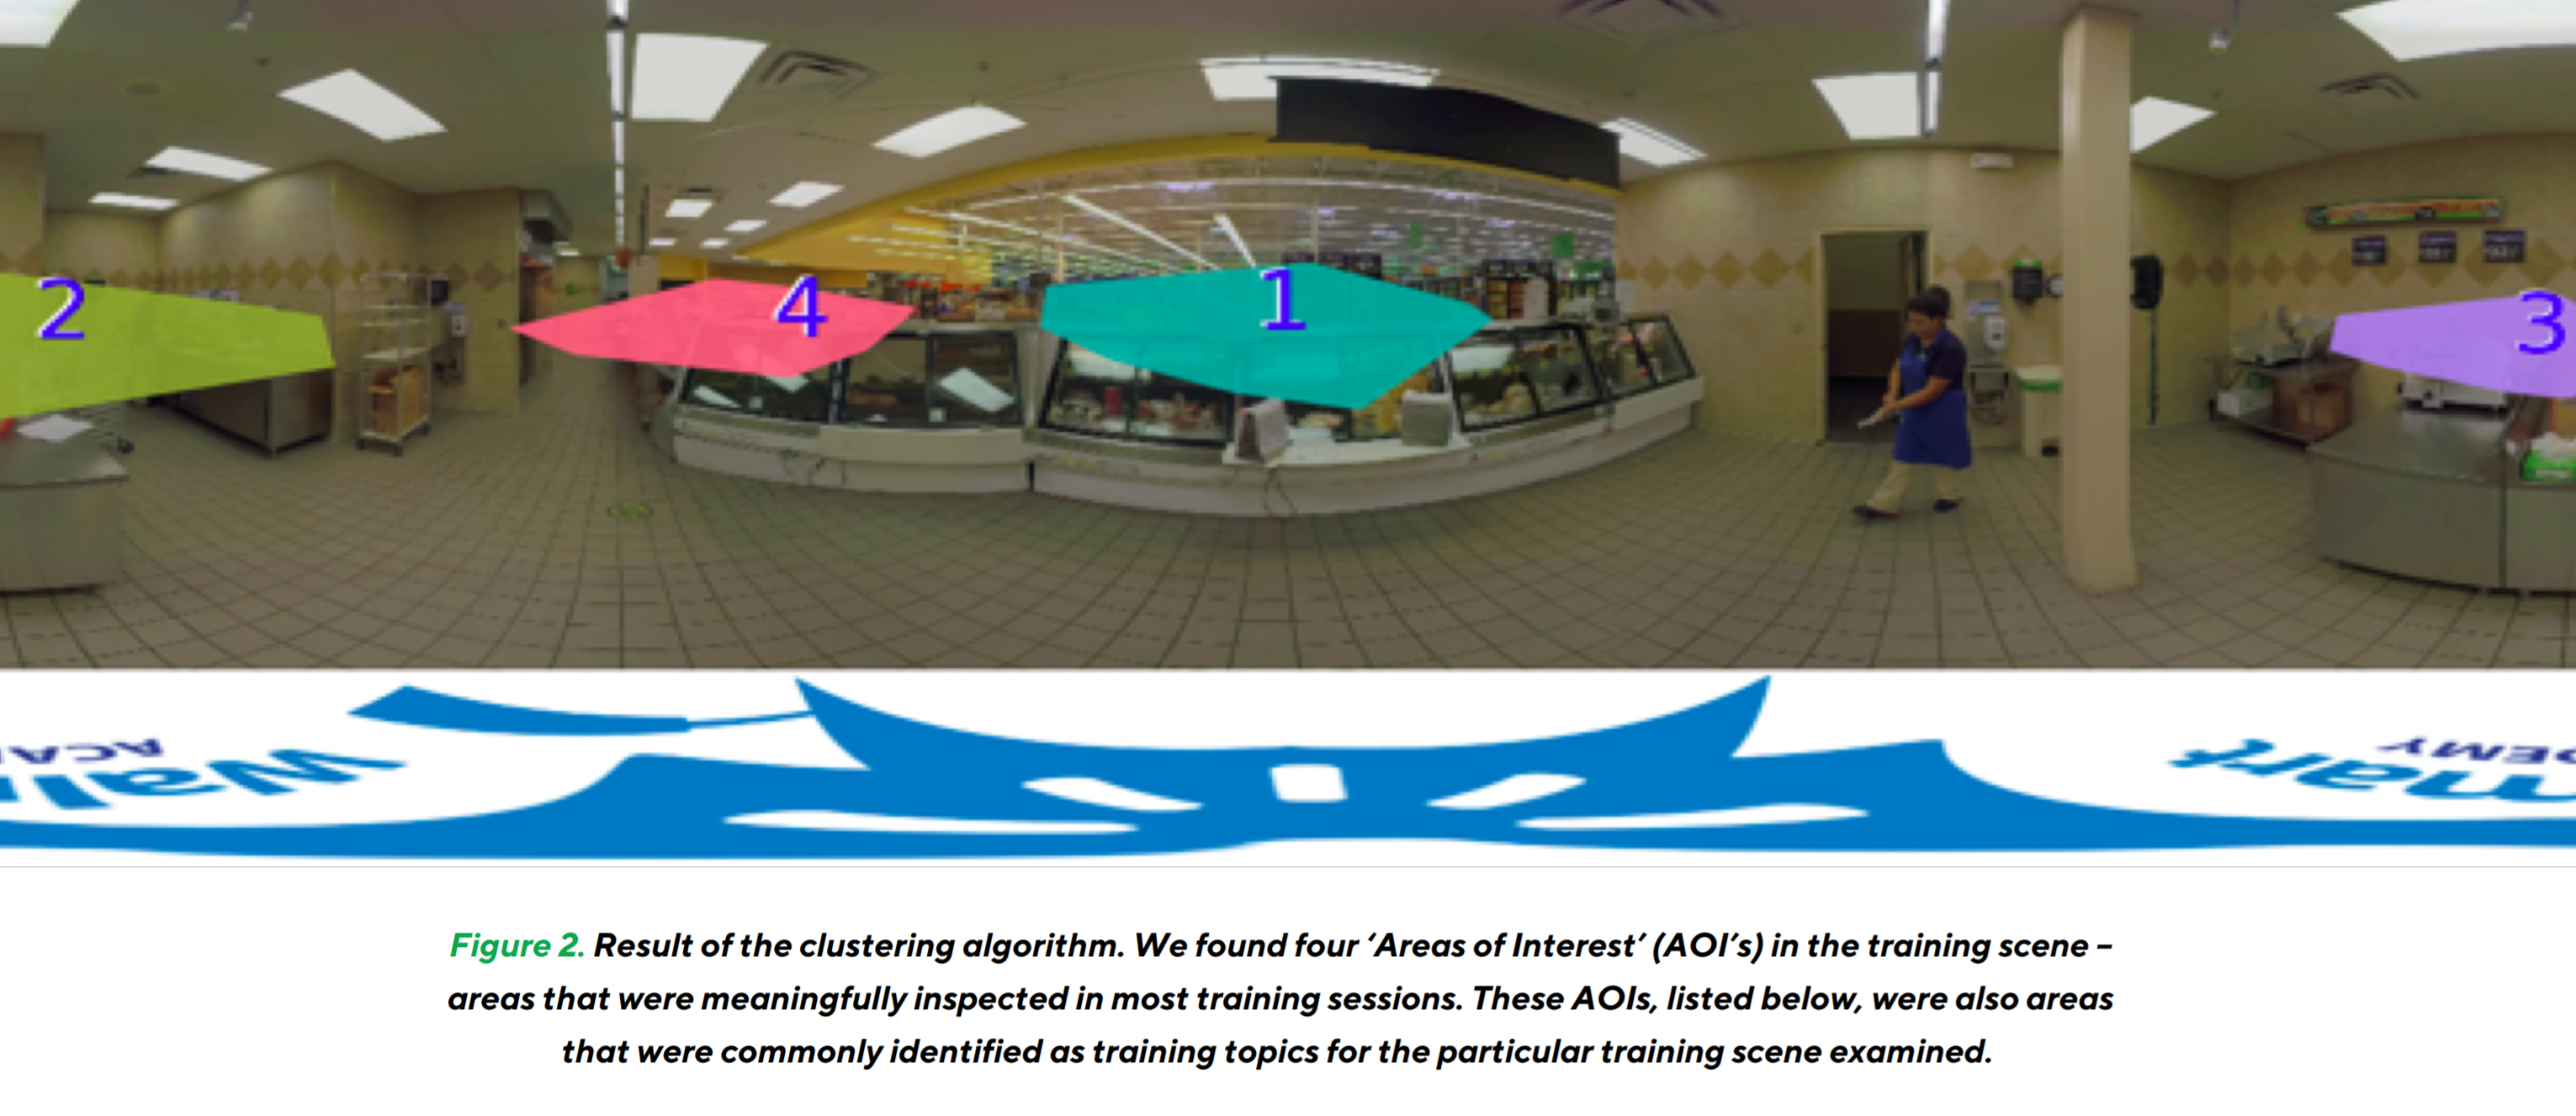
\includegraphics[width=\textwidth]{images/intentionanalys2.png}
\label{fig:intentionanalys2} 
\end{figure}

Neben den vielen Vorteilen existieren allerdings auch Nachteile, die nicht ignoriert werden sollten \citep{17}:

\begin{enumerate}
\item Beeinträchtigt die zwischenmenschlichen Kommunikation: das VR-Training könnte die Notwendigkeit der menschlichen Kommunikation reduzieren.
\item Mangel an Flexibilität: menschliche Kommunikation ist flexibel. Das VR-Training kann nicht für alle mögliche Aktivitäten Feedback geben.
\item Funktionsprobleme: Jede Software is anfällig für Fehler und Bugs. Solche Störungen können den Trainingsverlauf behindern.
\item Hohe Kosten: obwohl Google Cardboard eine günstige Alternative zu anderen VR-Techniken ist, kann nicht jedes Smartphone den hohen Rechenaufwand eines VR Programms bewältigen. Es benötigt demnach ein kompatibles Smartphone, welches im Preis teurer werden kann. Für PCs sind die Anforderungen bezüglich der Leistung noch höher.
\end{enumerate}\

\section{Stand der Technik}
 \subsection{Virtuelle Realität(VR)}
  \subsubsection{Technologie}
Carolina Cruz-Neira \citep{19} hat die technologieorientierte Definition von VR entwickelt \glqq Virtual Reality refers to immersive, interactive, multi-sensory, viewer-centered, three-dimensional computer generated environments and the combination of technologies required to build these environments.\grqq\
  
Die Implementierung der VR Technik liegt an der menschlichen Tiefenwahrnehmung, die auf der Fähigkeit zu \glqq stereoskopischem Sehen\grqq\ beruht \citep{20}. Die Augen übertragen die Bilder, die auf die Netzhaut abgebildet werden, zum Gehirn. Durch die Analyse auf die überlappende Teile der Bilder von linkem und rechtem Auge wird die Tiefenwahrnehmung erstellt, wodurch die Objekten dreidimensional erscheinen. (Abbildung ~\ref{fig:stereoskopischesSehen})

\begin{figure}[ht]
\vspace*{1em}
\centering
\caption{Stereoskopisches Sehen}
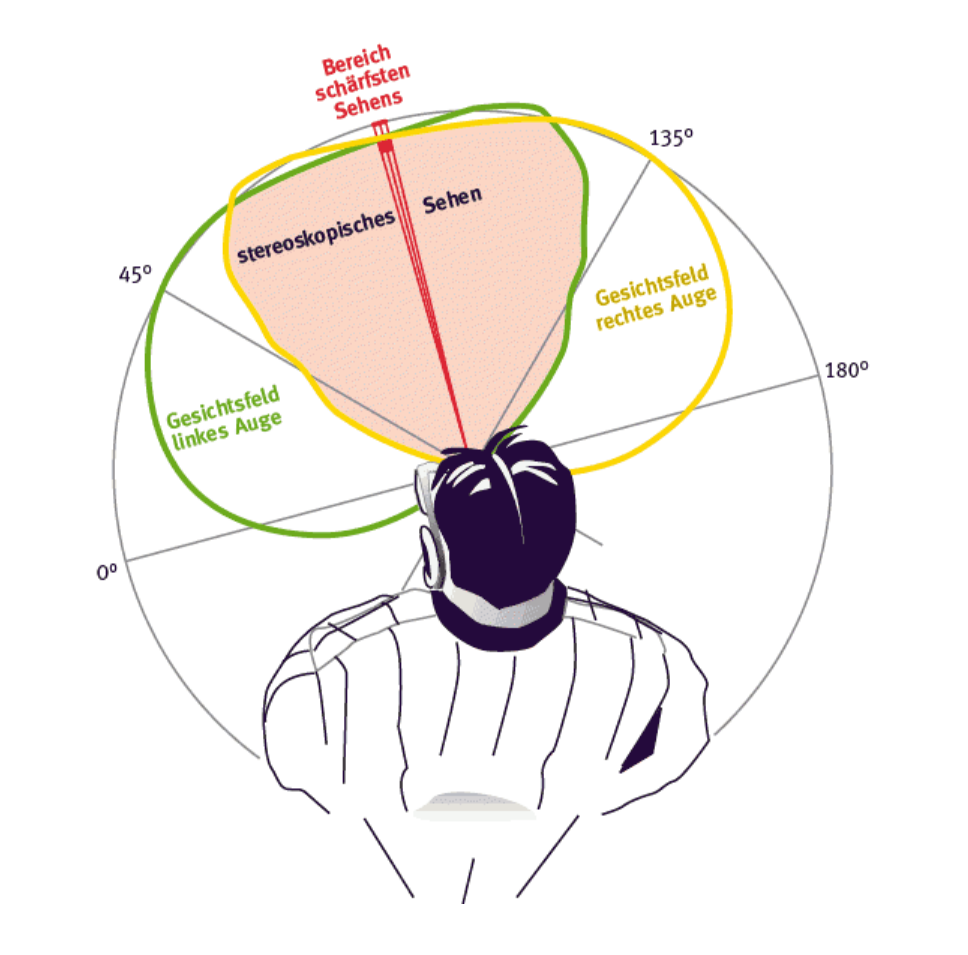
\includegraphics[width=\textwidth]{images/stereoskopischesSehen.png}
\label{fig:stereoskopischesSehen} 
\end{figure}

Bei HMDs (Head-Mounted Display) werden die Bilder entsprechend dem rechten und linken Auge angepasst und separat auf je einem Screen pro Auge dargestellt, sodass im gesamten der Eindruck eines zusammenhängenden Bildes entsteht. Das Gehirn leistet dabei die Arbeit, dass die Bilder passend zusammengesetzt werden und ein räumlicher Eindruck entsteht. Es entsteht somit ein dreidimensionales Szenario, in dem sich der Träger des HMDs befindet. (Abbildung ~\ref{fig:howToCreate})

\begin{figure}[ht]
\vspace*{1em}
\centering
\caption{Erstellung der stereoskopischen 3D Szene}
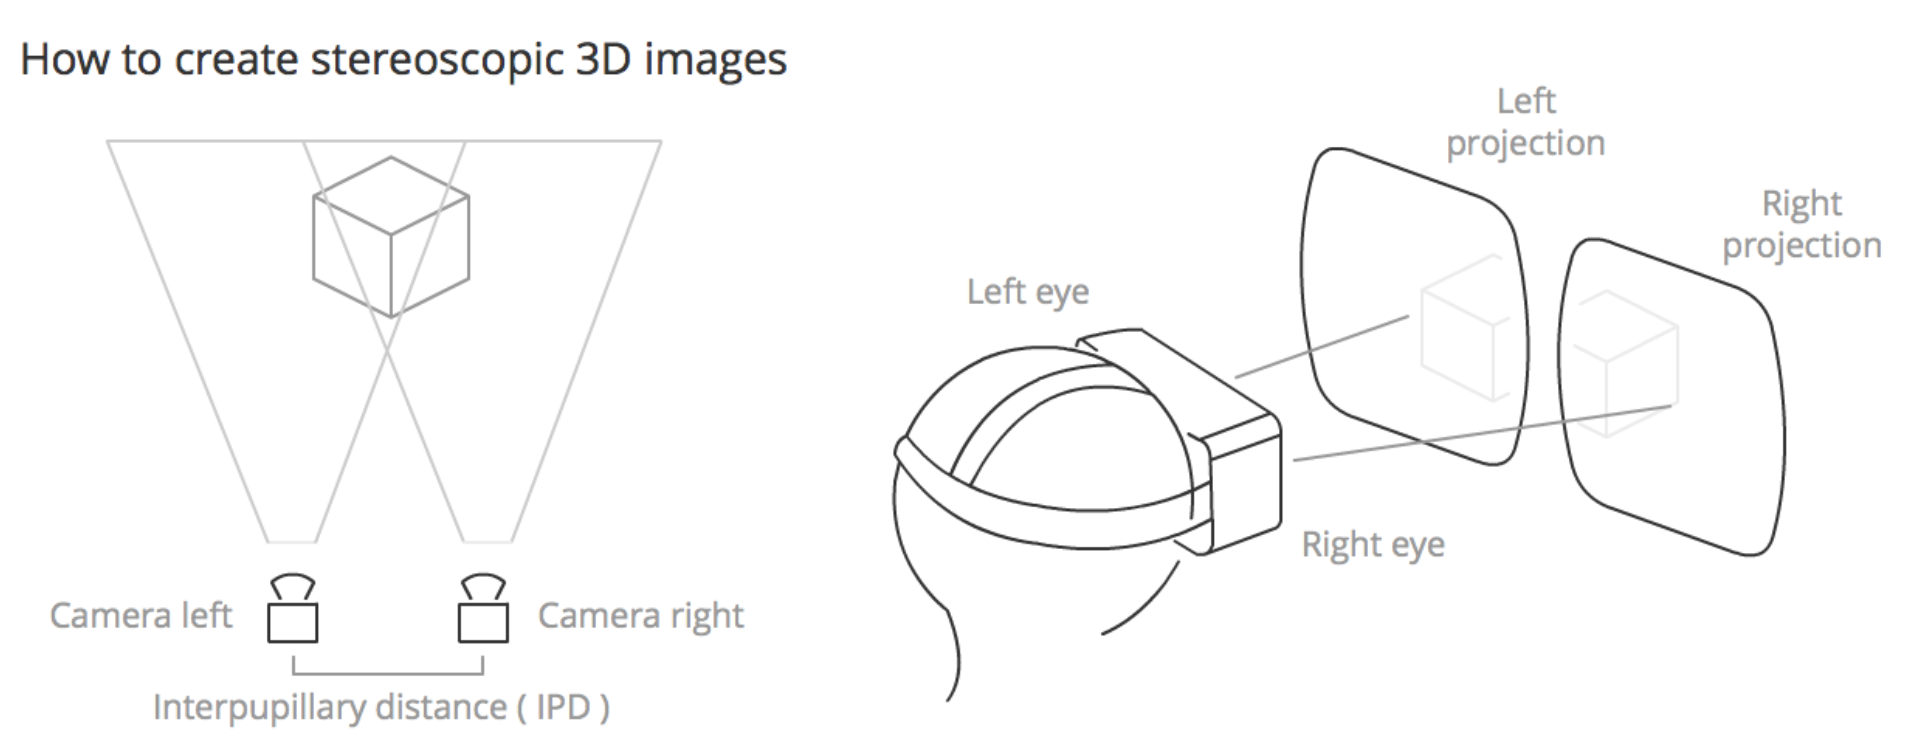
\includegraphics[width=\textwidth]{images/howToCreate.png}
\label{fig:howToCreate} 
\end{figure}

  \subsubsection{Geräte}
  Typische VR Geräte bestehen aus drei Teilen, dem HMD, einem Rechner und einem Controller/mehreren Controllern. Das HMD ist der Hauptteil der VR Geräte, wobei es unterschiedliche HMD-Typen gibt.
  
  Nach der Form des Rechners können HMDs in zwei Gruppen klassifiziert werden können: unmobile und mobile.
  
  Unmobile HMD bedeutet, dass der Rechner (Desktop oder Laptop) während der Ausführung der entsprechenden VR-Applikation, mit dem HMD per Kabel verbunden sein muss. Dazu gehören beispielsweise die Oculus Rift \citep{31} und die HTC Vive \citep{32}. Die Vorteile davon sind, dass die Rechenleistung hoch ist, die Kapazität der Speicher groß ist und die Wärmeableitung kräftig ist. Die Nachteile sind hohe Kosten, weil ein extra Rechner notwendig ist. Und die Netzteile für Rechner und HMD sind gefordert, deshalb ist die Bewegung während der Nutzung eingeschränkt.
  
  Mobile HMD bedeutet, dass sich der \glqq Rechner\grqq\ im HMD befindet oder im HMD integriert ist. Dieser Rechner ist normalerweise ein Smartphone. Dazu gehören beispielsweise Google Cardboard \citep{33}, Samsung Gear VR \citep{34}, Google Daydream VR \citep{35}. Die andere Variante ist, dass der Rechner integriert ist, deswegen ist ein extra Smartphone unnötig, z.B. Oculus Go \citep{36}. Die Vorteile der mobilen HMDs sind, dass die Größe der Geräte klein ist, das Netzteil während des Anwendens nicht gebraucht wird und der Preis ziemlich niedrig ist. Die Nachteile sind, dass die Leistung relativ schwach und die Kühlung kraftlos ist.
  
  Nach den Möglichkeiten der Bewegung können die HMDs in zwei Gruppe unterteilt werden, drei degrees of freedom (DoF) und sechs DoF.
  
  DoF beschreibt die \glqq Anzahl der Möglichkeiten\grqq\ eines Objekts in einem Raum. Es könnte als \glqq verschiedene grundlegende Möglichkeiten, wie sich ein Objekt bewegen kann\grqq\ erklärt werden \citep{25}. Es gibt insgesamt sechs DoF für HMDs, und sie können in zwei verschiedene Typen unterteilt werden: Translation und Rotation.
  
  Translation bedeutet räumliche Bewegung in einem Raum. Das Objekt kann auf drei Achsen bewegt werden. Die drei Achsen gelten als drei \glqq degree of freedom\grqq. (Abbildung ~\ref{fig:translationRotation})
  
  Eine Rotation bedeutet eine kreisförmige Drehung um eine bestimmte Achse. Das Objekt kann auch auf drei Achsen gedreht werden, die als die anderen drei \glqq degree of freedom\grqq\ gelten. (Abbildung ~\ref{fig:translationRotation})

\begin{figure}[ht]
\vspace*{1em}
\centering
\caption{Translation \& Rotation}
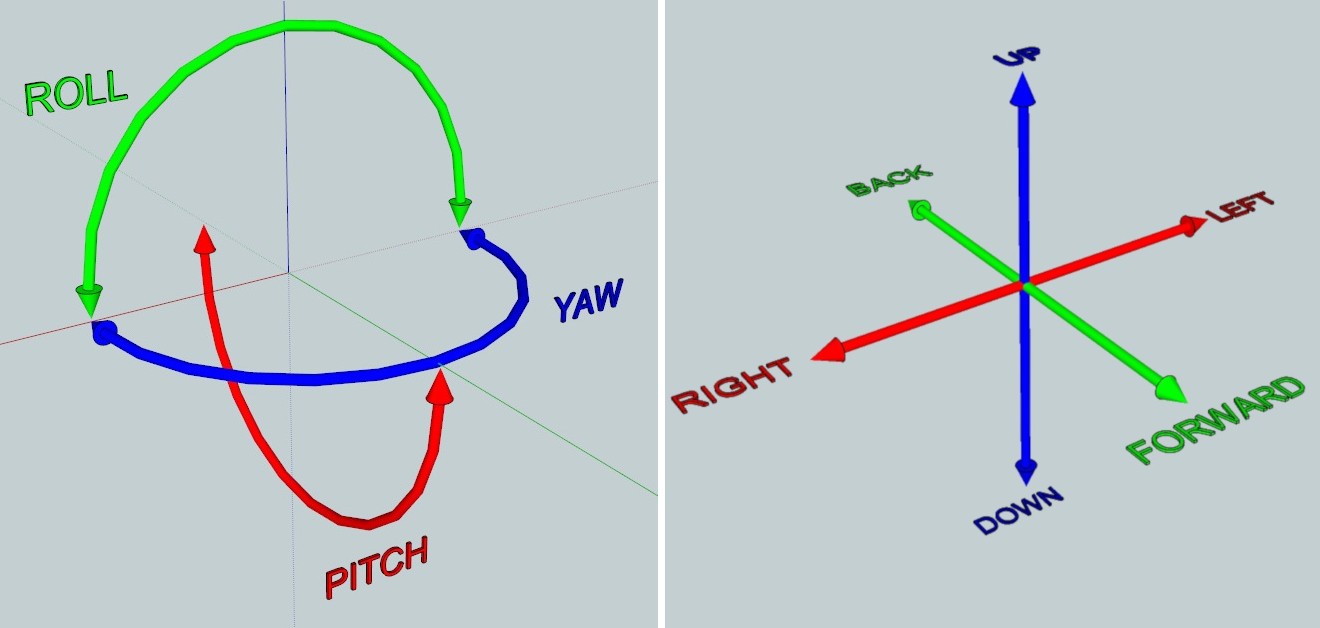
\includegraphics[width=\textwidth]{images/translationRotation.png}
\label{fig:translationRotation} 
\end{figure}
  
  Wenn ein HMD drei DoF hat, kann es normalerweise nur die Rotationen erkennen. Wegen der Begrenzung der Leistung ist erfahrungsmäßig ein mobile HMD ein HMD mit drei DoF.
  
  Im Vergleich zu HMDs mit drei DoF, kann ein HMD mit sechs DoF nicht nur die Rotationen sondern auch die Translationen erkennen und umsetzen. Durch einen externen starken Rechner kann die unmobile HMD diese aufwendigen Berechnnungen bewältigen. (Abbildung ~\ref{fig:6DoF-vs-3DoF})
  
\begin{figure}[ht]
\vspace*{1em}
\centering
\caption{3 DoF \& 6 DoF}
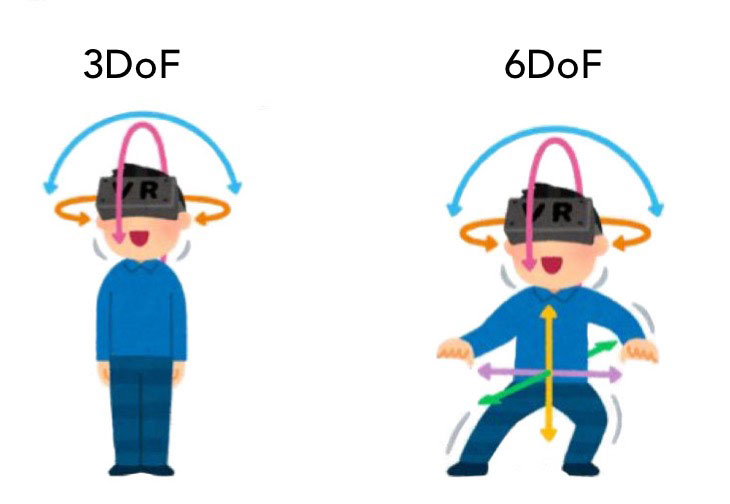
\includegraphics[width=\textwidth]{images/6DoF-vs-3DoF.jpg}
\label{fig:6DoF-vs-3DoF} 
\end{figure}
  
  Theoretisch wird ein Controller mit drei DoF z.B. Gear VR Controller und Daydream VR Controller für ein HMD mit drei DoF ausgestattet. Die Position von Controllern mit drei DoF in dem Raum ist fest. Die Interaktion zwischen den Objekten und dem Controller wird durch einem von Controller strahlenden Raycaster aufgerufen. (Abbildung ~\ref{fig:3dcontroller})

\begin{figure}[ht]
\vspace*{1em}
\centering
\caption{3 DoF Daydream Controller}
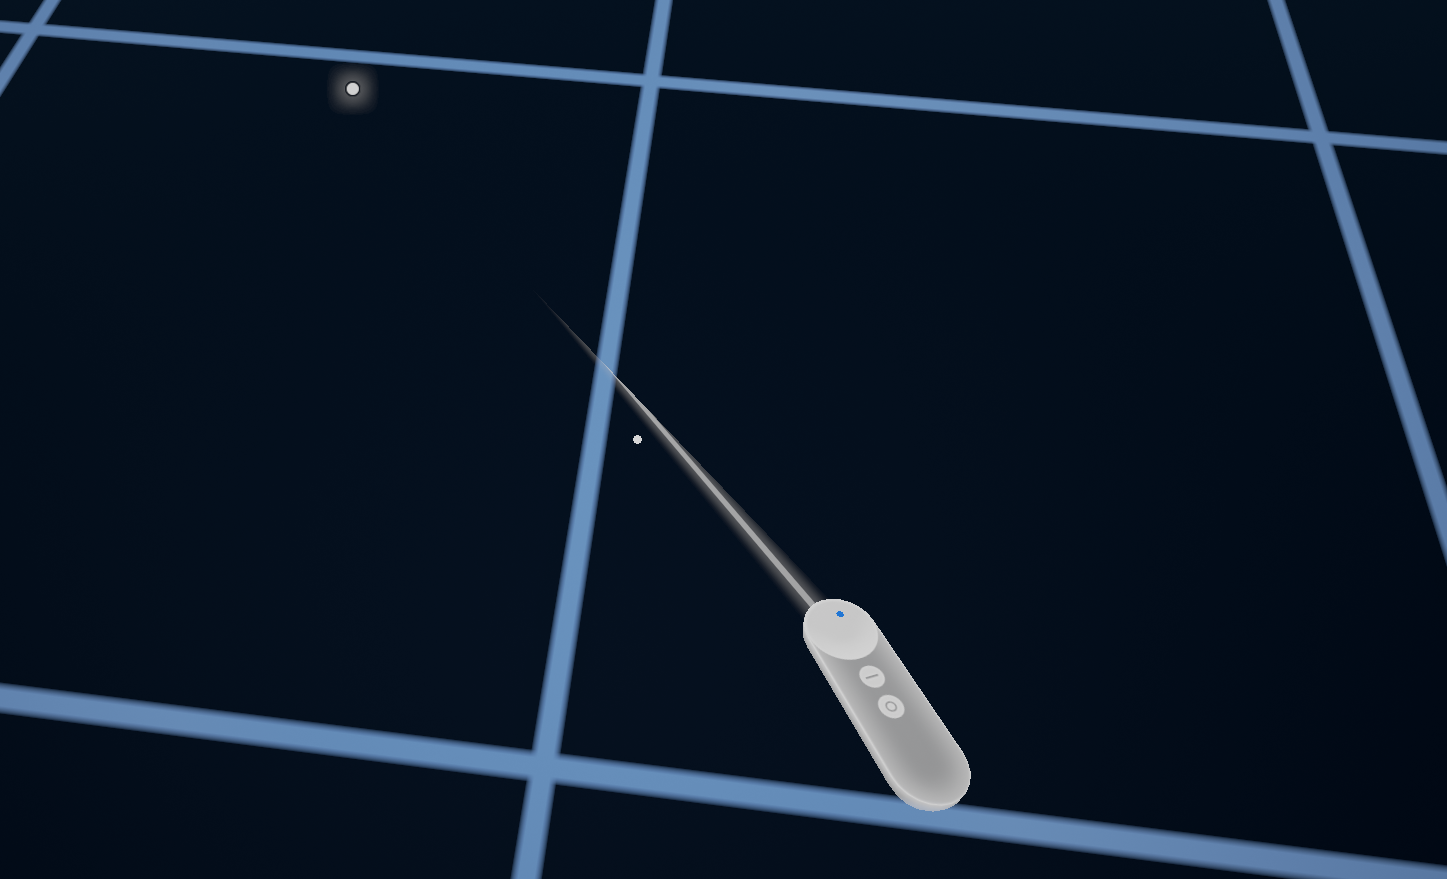
\includegraphics[width=\textwidth]{images/3dControllerDaydream.png}
\label{fig:3dcontroller} 
\end{figure}

  Es gibt auch HMD wie Google Cardboard und die ältere Version der Gear VR, die keine zugehörigen Controller haben. Normalerweise steht ein Knopf oder ein Trackpad an der Seite des HMDs für Interaktion zu Verfügung.
  
  Controller mit sechs DoF werden mit somit zusammen mit HMD mit sechs DoF benutzt. Es bietet die größtmögliche interaktive Freiheit in einem Raum. (Abbildung ~\ref{fig:6dcontroller})
  
\begin{figure}[ht]
\vspace*{1em}
\centering
\caption{Bewegung mit HTC Vive}
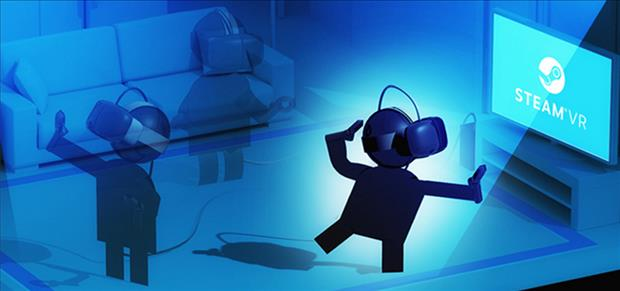
\includegraphics[width=\textwidth]{images/6dcontroller.jpg}
\label{fig:6dcontroller} 
\end{figure}

\begin{figure}[ht]
\vspace*{1em}
\centering
\caption{VR Geräte}
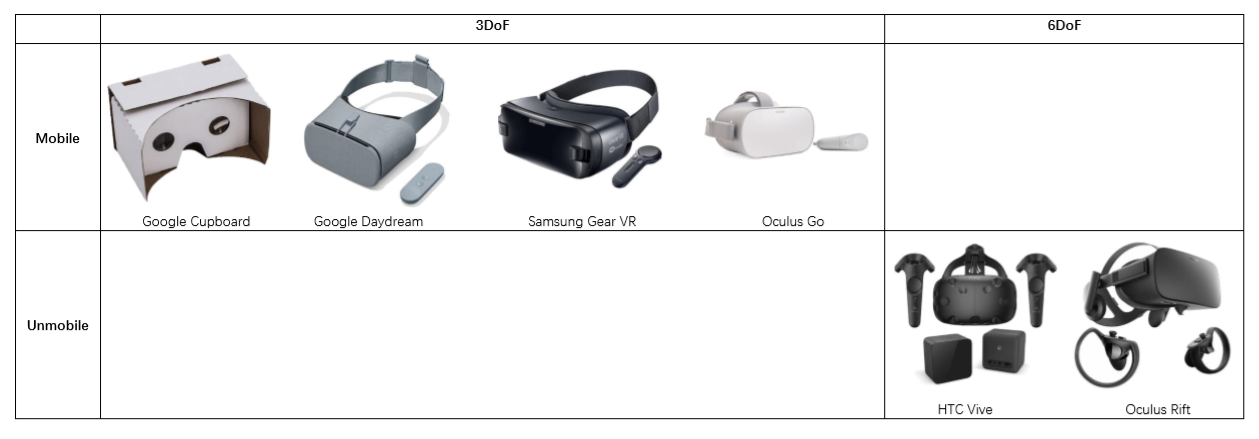
\includegraphics[width=\textwidth]{images/vrDevicesTableCorrect.png}
\label{fig:vrDevicesTable} 
\end{figure}
  
  \subsubsection{Entwicklung}
  Obwohl Unity und Unreal Engine ursprünglich Game Engines sind, spielen beide eine wichtige Rollen im Bereich VR Entwicklung. Mit den Engines können VR Projekte einfach erstellt, entwickelt und debuggt werden. Bei der Erstellung wird die Grundstruktur des Projekts aufgebaut. Während der Entwicklung stehen viele vorgefertigte Funktionen wie Kollisionserkennung und Physik-Simulationen zu Verfügung. Die Standard IDE (Integrated Development Environment) ist Visual Studio von Microsoft. Aber es ist möglich, eine andere IDE zu benutzen. Wegen der engen Verbindung zwischen Visual Studio und den beiden Engines ist Debuggen durch \glqq Checkpoint \grqq\ und \glqq Breakpoint\grqq\ mühelos. Mit Game Engines können Projekte als anpassende Formate für unterschiedliche Geräte erstellt werden.

  C\# ist die bevorzugte Programmiersprache für Unity, die von Microsoft entwickelt wurde. Eine andre Möglichkeit ist Unity Script, eine Variante von JavaScript, die etwas anfängerfreundlicher als C\# ist . (Abbildung ~\ref{fig:unity})
  
\begin{figure}[ht]
\vspace*{1em}
\centering
\caption{Entwickelung mit Unity}
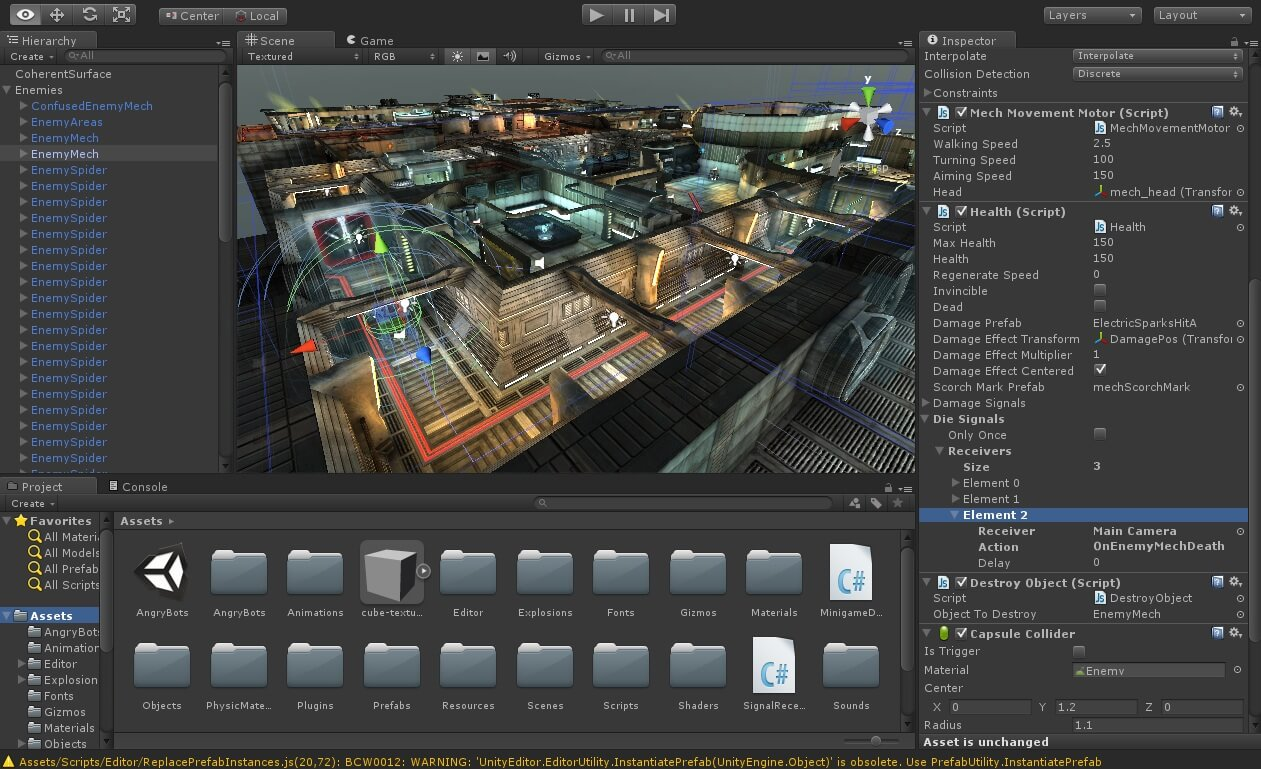
\includegraphics[width=\textwidth]{images/unity.jpg}
\label{fig:unity} 
\end{figure}
  
  C++ ist die Standard Programmiersprache bei der Unreal Engine (Abbildung ~\ref{fig:uec}). Außerdem wird Blueprints Visual Scripting unterstützt (Abbildung ~\ref{fig:ueblueprint}). Das ist eine grafische knotenbasierte Schnittstelle, um die Interaktion eines Objekts zu definieren. Die Option macht es möglich, dass die Entwickler ohne große Programmierkenntnisse ein Skript in Unreal Engine schreiben können.

\begin{figure}[ht]
\vspace*{1em}
\centering
\caption{Entwickelung mit Unreal Engine}
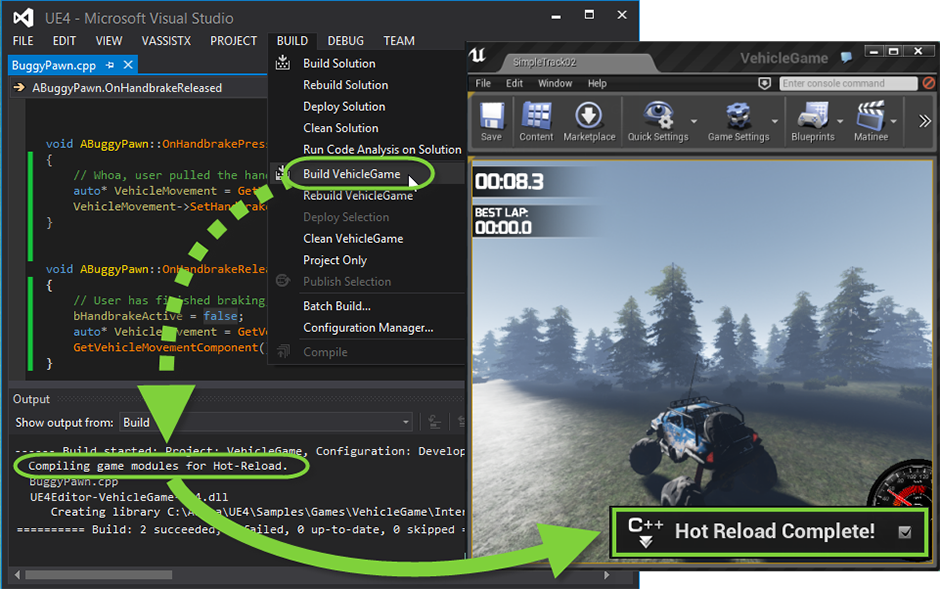
\includegraphics[width=\textwidth]{images/uec.png}
\label{fig:uec} 
\end{figure} 
  
\begin{figure}[ht]
\vspace*{1em}
\centering
\caption{Blueprint bei Unreal Engine}
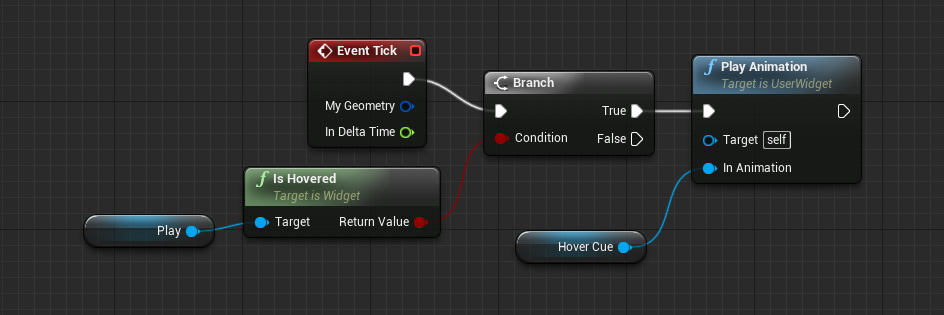
\includegraphics[width=\textwidth]{images/ueblueprint.png}
\label{fig:ueblueprint} 
\end{figure}
  
 \subsection{WebVR}
 Um \glqq WebVR \grqq\ besser zu verstehen, werden zwei relevante Begriffe erklärt, native Applikation (native App) und webbasierte Applikation (Web App).
 
 Native Apps werden speziell für ein Betriebssystem, z.B. IOS, Android, Macintosh und Windows programmiert und laufen dann ausschließlich auf den entsprechenden Geräten. Der Vorteil ist, \glqq dass alle Schnittstellen zu Hardware einheitlich funktionieren und die Ressourcen des Geräts optimal genutzt werden\grqq\ \citep{22}. Die Nachteile sind, dass der Aufwand der Entwicklung hoch ist, weil für jedes Betriebssystem eine bestimmte Version entwickelt werden muss. Außerdem muss die native App vor dem Anwendung heruntergeladen und installiert werden.
 
 Web Apps werden für Browser entwickelt. Das heißt, dass sie im Browser laufen und unabhängig vom Betriebssystem sind. Der Vorteil ist die gute Erreichbarkeit. Der Aufruf ist durch die Angabe einer URL im Browser, und Herunterladen und Installation sind nicht von Nöten. Die Nachteile sind die Abhängigkeit von Internet und schwächerer Leistung als native Apps.
 
  \subsubsection{Technologie}
 WebVR ist ein Form von Web App. \glqq WebVR is an open specification that makes it possible to experience VR in your browser. The goal is to make it easier for everyone to get into VR experiences, no matter what device you have. \grqq\ \citep{21} Ein wichtiges Merkmal ist, dass die Szenarien nicht nur in VR Form auf HMDs, sondern auch als 3D Form über den normalen flachen Bildschirm dargestellt werden können, wenn keine VR Geräte zur Verfügung stehen.
 
 Obwohl zur Zeit WebVR noch nicht von allen Browsern unterstützt wird, hat WebVR eine ziemlich breite Zugänglichkeit. (Abbildung ~\ref{fig:supportedBrowsers})
 
\begin{figure}[ht]
\vspace*{1em}
\centering
\caption{Unterstützte Browser}
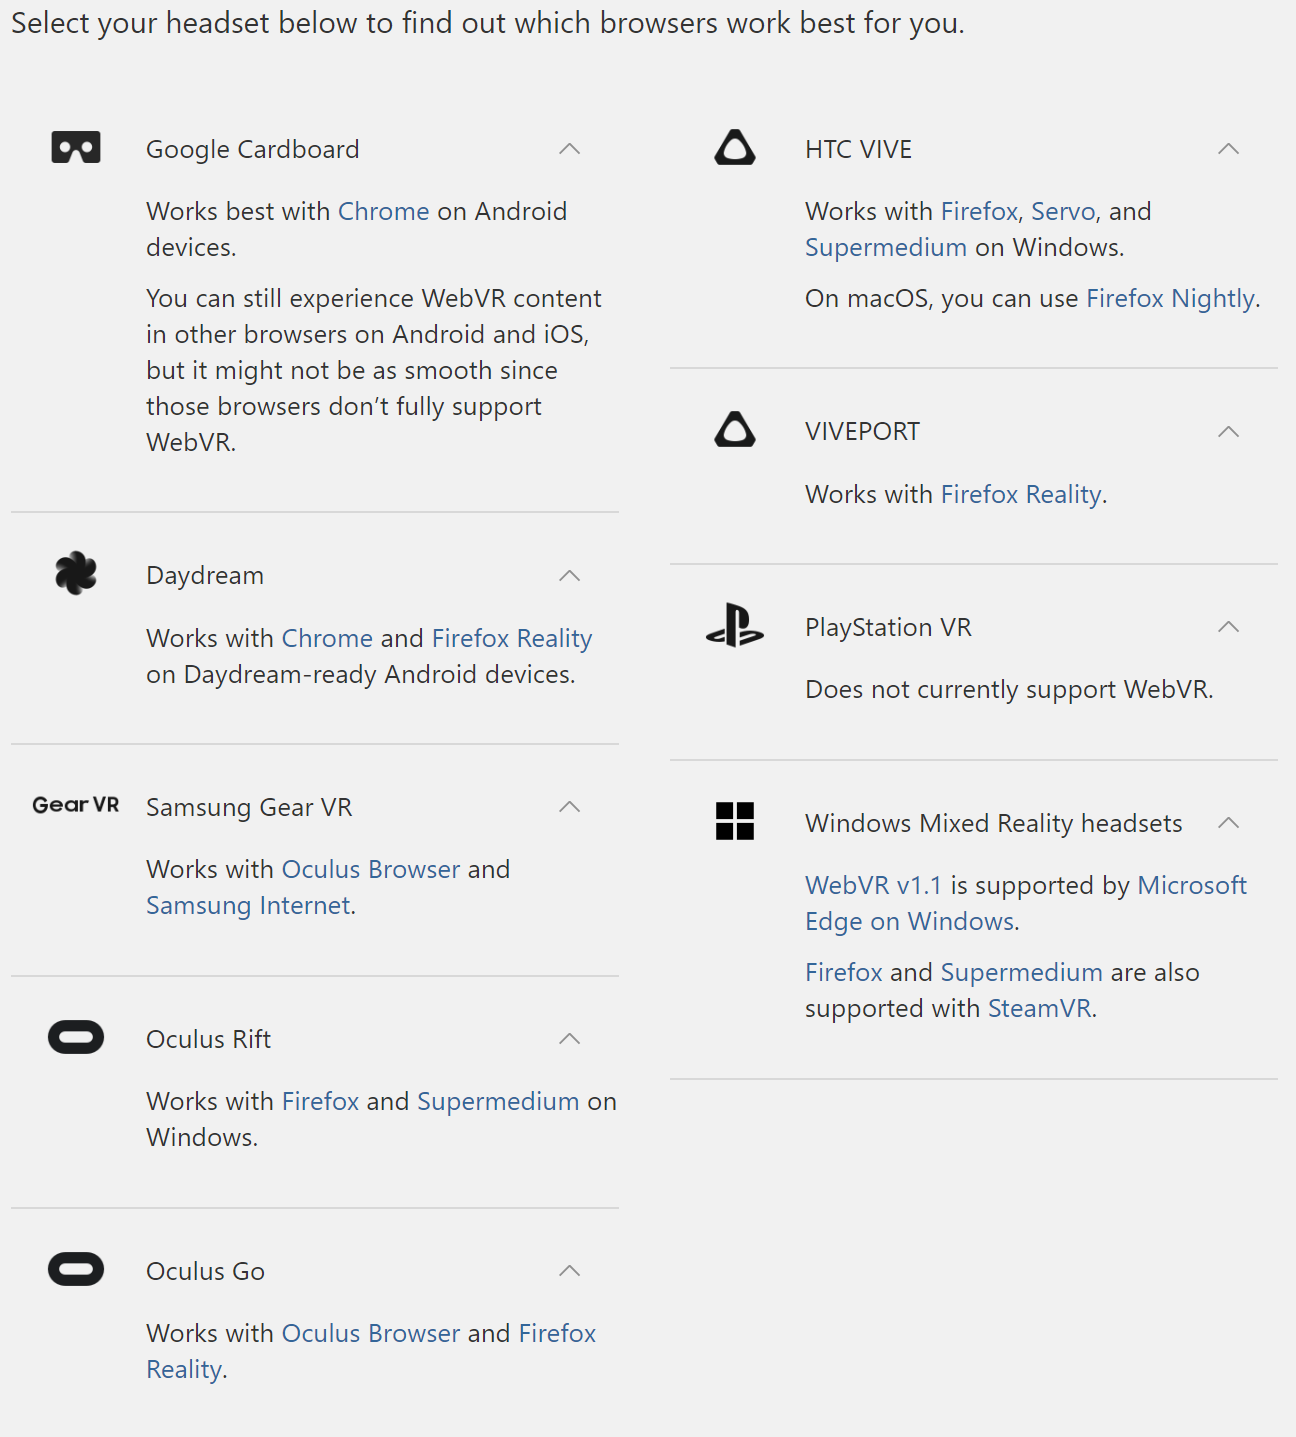
\includegraphics[width=\textwidth]{images/supportedBrowsers.png}
\label{fig:supportedBrowsers} 
\end{figure}
 
  \subsubsection{Entwicklung}
 Die Grundtechnik von WebVR ist WebGL, die auf OpenGL basiert. OpenGL ist eine Application Programming Interface (API), um 2D und 3D Grafiken darzustellen. \glqq WebGL is a cross-platform, royalty-free web standard for a low-level 3D graphics API based on OpenGL ES, exposed to ECMAScript via the HTML5 Canvas element. \grqq\ \citep{23} Das heißt, dass die Grafiken durch WebGL in eine Form umgewandelt werden, die ein Browser verstehen kann. 
 
 Die Programmierung erfolgt direkt mit WebGL, was allerdings kompliziert und zeitaufwendig ist. Um effizienter zu entwickeln werden erfahrungsmäßig Javascript 3D Engines benutzt, z.B. three.js, PlayCanvas und Unity.
 
 Die three.js ist eine open source JavaScript Bibiliothek, die die WebGL Objekte beinhaltet. Durch den Funktionen von three.js Objekten können die WebGL Objekte modifiziert werden. Die Funktionsweise ist änhlich wie JQuery zu JavaScript. Auf three.js werden unterschiedliche Frameworks beispielsweise A-Frame, React 360 und Vizor entwickelt.
 
 PlayCanvas ist eine webbasierte visuelle Entwicklungsplattform für interaktive Inhalte im Web. Die Entwicklung wird im Browser durchgeführt.
 
 Mit Unity WebVR Assets von Mozilla kann das Unity Projekt als WebVR gebildet werden.

\begin{figure}[ht]
\vspace*{1em}
\centering
\caption{Struktur der Technologie von WebVR}
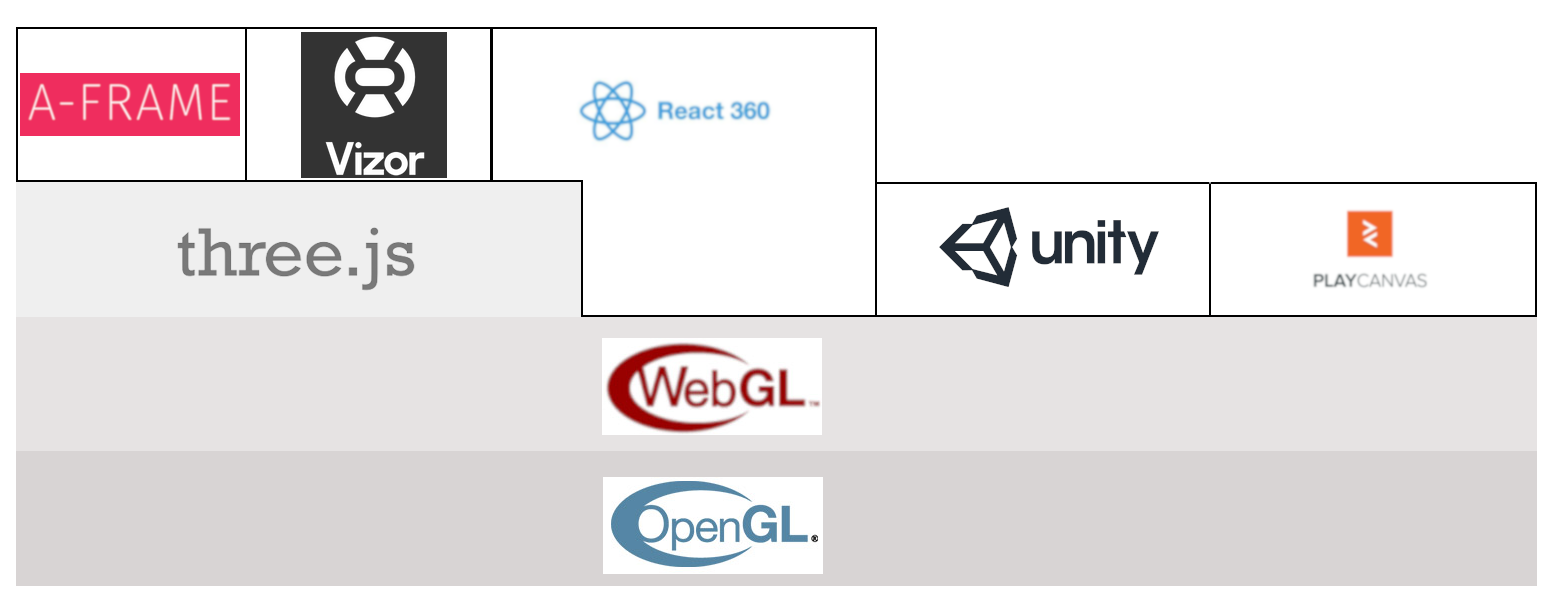
\includegraphics[width=\textwidth]{images/webVRStruckture.png}
\label{fig:webVRStruckture} 
\end{figure}

\section{Zusammenfassung}
Der Stand der Forschung bietet die theoretische Unterstützung für die Konzeption von diesem Projekt. Hier werden die Aspekte der Kritiken in diesem Kapitel aufgelistet. Im Vergleich mit dem Real Skillslab haben E-Learning und VR-Training eigne Vorteile und Nachteile. Durch die Verbindung zwischen WebVR und Learning Management System ist es möglich, durch die Ergänzung die Nachteile von beiden zu vermeiden oder erleichtern. (Abbildung ~\ref{fig:standDerForschungTabelle})

\begin{figure}[ht]
\vspace*{1em}
\centering
\caption{Vergleich der unterschiedlichen Lerntechnologien}
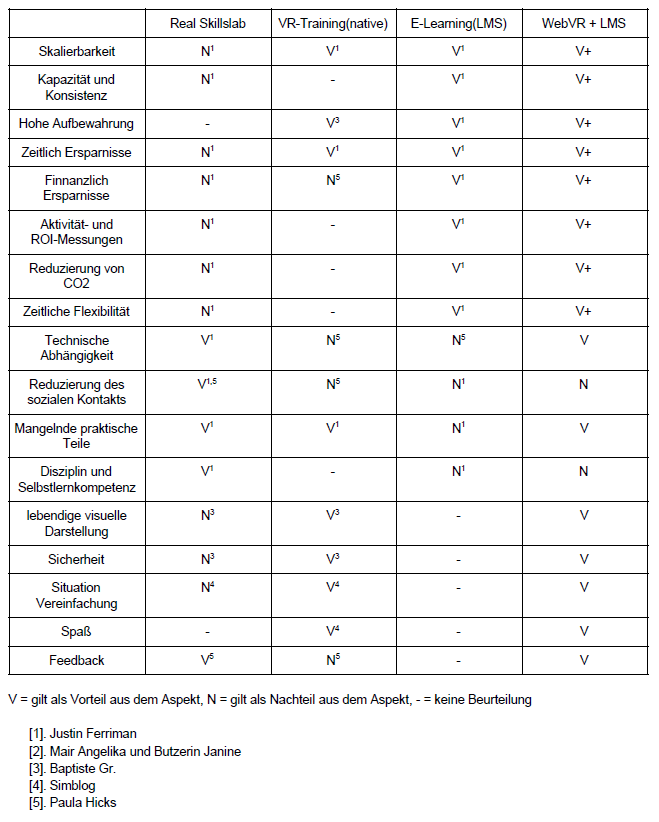
\includegraphics[width=\textwidth]{images/standDerForschungTabelle.png}
\label{fig:standDerForschungTabelle} 
\end{figure}

Die WebVR Technik ist noch ziemlich junge Technik. Allerdings bietet WebVR die Möglichkeit, webbasiert cross-platform VR Projekt zu implementieren und das VR-Training im Bereich E-Learning bringen.



